

{
	\renewcommand{\secimage}{./media/aesthetics/S2}
	\section{Modeling our Model}
}

\subsection{Coulomb Gas}

\begin{frame}
	\only<5->{\vspace{0.39cm}}
	We know that
	\only<1-4>{
		\begin{equation*}
			p_n(\{z_i\}_{i=1}^n) = p\left( \eigenvalues \right) = \frac{1}{\pZ{n}{Q}} \prod_ {i < j}^n |z_i - z_j|^2 \prod_{j=1}^{n} \ee^{- n \Q(z_j)} 
		\end{equation*}
	}
	\only<1-4>{
		\visible<2-4>{
	We can notice two effects, one coming from the Jacobian and the other one from $Q$.	
		\begin{equation*}
			p_n\left( \eigenvalues \right) >
			\begin{cases}
				\visible<3->{
				p_n\left( \eigenvaluesclose \right), \quad \text{the interactions dominates.} \\
				\\
				}
				\visible<4>{
				p_n\left( \eigenvaluesfar \right), \quad \text{the external potential dominates$.^*$}
			}
			\end{cases}
	\end{equation*}
}
	}
	\only<5->{
		\vspace{0.159cm}
		\begin{align*}
			& p_n(\{z_i\}_{i=1}^n) = p\left( \eigenvalues \right) = \frac{1}{\pZ{n}{Q}} \prod_ {i < j}^n |z_i - z_j|^2 \prod_{j=1}^{n} \ee^{- n \Q(z_j)}  \\
			\visible<6->{& = \frac{1}{\pZ{n}{Q}} \exp\left\{- n^2 \left( \frac{1}{n} \sum_{i = 1}^{n} \Q(z_i) + \frac{1}{n^2} \sum_{i \neq j} \ln |z_i - z_j| \right) \right\} \\}
			\visible<7->{& = \frac{\ee^{-n^2 \Hf(\chi_n)}}{\pZ{n}{Q}}, \quad  \Hf(\chi_n) = \frac{1}{n} \sum_{i = 1}^{n} \Q(z_i) + \frac{1}{n^2} \sum_{i \neq j}^{n} \ln |z_i - z_j| }
		\end{align*}
		\visible<8->{The measure $\dd p_n$ models an Coulomb-interacting gas of charged indistinguishable particles under some external field $\Q$ on $\C$.}
		\vspace{1cm}
		
		\visible<9->{If we want to study this gases, how to describe its statistical properties?}
		\vspace{1.5cm}
	}
\end{frame}

\subsection{Point Process}

\begin{frame}{Point Process}
	\only<3-5>{
		\vspace{0.20cm}
	}
	Suppose there are $n$ particles at random locations in the complex plane $\C$ denoted by the configuration $\chi_n = \set{\mmany{z}{n}}$. 
	\begin{center}
	\vspace{-0.7cm}
	\begin{tikzpicture}
		\begin{axis}[axis line style={opacity=0}, ticks=none,
			xmin=-1.5, xmax=1.5,
			ymin=-1.5, ymax=1.5,
			xticklabel pos=top,
			scatter/classes={%
				a={ mark size=0.5pt}}
			]
			\addplot[skip coords between index={100}{500}, opacity=1, scatter, mark=x, black, only marks] table [col sep=comma] {./media/aesthetics/5lines/a2t0.csv};
			\only<3>{
			\draw[color = red] plot[smooth cycle] coordinates {(60,60) (85,100) (67,170) (120,150) (120,60)};
			}
			\only<4>{
			\draw[color = blue] plot[smooth cycle] coordinates {(160,200) (170,240) (150,260) (225,235) (280,200) (260, 180) (215, 200)};
			}
			\only<5>{
			\draw[color = teal] plot[smooth cycle] coordinates {(110,110) (100,160) (160,240) (135,155) (145,140)};
			}
		\end{axis}
	\end{tikzpicture}
	\vspace{-0.9cm}
	\end{center}	
	\visible<2->{Define a quantity \only<2,6->{$\xi(A)$}\only<3>{$\xi(\textcolor{red}{A_1})$}\only<4>{$\xi(\textcolor{blue}{A_2})$}\only<5>{$\xi(\textcolor{teal}{A_3})$} s.t.
	\begin{equation*}
		\only<2,6->{\xi(A)}\only<3>{\xi(\textcolor{red}{A_1})}\only<4>{\xi(\textcolor{blue}{A_2})}\only<5>{\xi(\textcolor{teal}{A_3})}=\sum_{k=1}^{n}\delta_{\only<3>{\textcolor{red}{A_1}}\only<4>{\textcolor{blue}{A_2}}\only<5>{\textcolor{teal}{A_3}}}(z_k)\only<3>{=\textcolor{red}{21}}\only<4>{=\textcolor{blue}{9}}\only<5>{=\textcolor{teal}{10}}
	\end{equation*}
	\visible<6->{
	This defines a \textit{random counting measure} in the usual sense. \visible<7->{A \textbf{point process} $\mathbb{P}$ on $\C$ is a probability measure on the space of all counting measures $\mathcal{N}(\C)$.}
	}
	}
	\vfill
\end{frame}

\begin{frame}
	Consider the configuration $\only<1-2,6->{\chi_n = \set{\mmany{z}{n}}}\only<3>{\chi^{(1)}_n = \set{\mmany{z^{(1)}}{n}}} \only<4>{\chi^{(2)}_n = \set{\mmany{z^{(2)}}{n}}} \only<5>{\chi^{(3)}_n = \set{\mmany{z^{(3)}}{n}}}$.
	\vspace{-0.5cm}
	\begin{columns}
	\begin{column}{0.4\textwidth}  %%<--- here
		\hspace{2cm}
		\begin{center}
		\begin{tikzpicture}
			\begin{axis}[axis line style={opacity=0}, ticks=none,
				xmin=-1.5, xmax=1.5,
				ymin=-1.5, ymax=1.5,
				xticklabel pos=top,
				scatter/classes={%
					a={ mark size=0.5pt}}
				]
				\only<1-2>{
					\addplot[skip coords between index={0}{0}, skip coords between index={100}{500}, opacity=1, scatter, mark=x, black, only marks] table [col sep=comma] {./media/aesthetics/5lines/a2t0.csv};
				}
				\only<3>{
					\addplot[skip coords between index={0}{99}, skip coords between index={200}{500}, opacity=1, scatter, mark=x, black, only marks] table [col sep=comma] {./media/aesthetics/5lines/a2t0.csv};
				}
				\only<4>{
					\addplot[skip coords between index={0}{199}, skip coords between index={300}{500}, opacity=1, scatter, mark=x, black, only marks] table [col sep=comma] {./media/aesthetics/5lines/a2t0.csv};
				}
				\only<5-6>{
					\addplot[skip coords between index={0}{299}, skip coords between index={400}{500}, opacity=1, scatter, mark=x, black, only marks] table [col sep=comma] {./media/aesthetics/5lines/a2t0.csv};
				}
				\only<7->{
					\addplot[opacity=0.07, scatter, mark=*,draw opacity=0,black, only marks] table [col sep=comma] {./media/aesthetics/5lines/a2t0.csv};
				}
				\only<2->{
					\draw[color = red] plot[smooth cycle] coordinates {(60,60) (85,100) (67,170) (120,150) (120,60)};
				}
			\end{axis}
		\end{tikzpicture}
		\end{center}
	\end{column}
		\begin{column}{0.6\textwidth}  %%<--- here
		\begin{equation*}
			\only<2->{\only<2,6->{\xi}\only<3>{\xi^{(1)}}\only<4>{\xi^{(2)}}\only<5>{\xi^{(3)}} (\textcolor{red}{A_1}) = \sum_{k=1}^{n} \delta_{\textcolor{red}{A_1}}(\only<2,6->{z_k}\only<3>{z^{(1)}_k}\only<4>{z^{(2)}_k}\only<5>{z^{(3)}_k})}
		\end{equation*}
	\end{column}
	\end{columns}
	\visible<6->{
	We define
	\begin{equation*}
		\mathfrak{p}(A) \deff \E[\xi(A)] = \E[\#(\chi_n \cap A)], \quad A \in \mathcal{E}.
	\end{equation*} 
	\visible<7->{We will assume the existence of a function $\p_1(z)$ s.t.
		\begin{equation*}
			\mathfrak{p}(A) = \int_A \p_1(z) \dd^2 z
		\end{equation*}
		where $\dd^2 z$ is the usual area measure.} \visible<8->{The \textbf{$1$-point correlation function} $\p_1$  represents the infinitesimal probability of a point of the process being at a location $z$, i.e. $\mathbb{P}(\xi(\dd^2 z) = 1) = \p_1(z) \dd^2 z$.}
	}
\end{frame}

\begin{frame}
	\only<1>{
	\begin{center}
	\begin{tikzpicture}
		\begin{axis}[axis line style={opacity=0}, ticks=none,
			xmin=-1.5, xmax=1.5,
			ymin=-1.5, ymax=1.5,
			xticklabel pos=top,
			scatter/classes={%
				a={ mark size=0.5pt}}
			]
			\addplot[skip coords between index={100}{500}, opacity=1, scatter, mark=x, black, only marks] table [col sep=comma] {./media/aesthetics/5lines/a2t0.csv};
		\end{axis}
	\end{tikzpicture}
	\end{center}
	}
	\only<2>{
		\begin{center}
			\begin{tikzpicture}
				\begin{axis}[axis line style={opacity=0}, ticks=none,
					xmin=-1.5, xmax=1.5,
					ymin=-1.5, ymax=1.5,
					xticklabel pos=top,
					scatter/classes={%
						a={ mark size=0.5pt}}
					]
					\addplot[opacity=1, scatter, mark=x, black, only marks] table [col sep=comma] {./media/aesthetics/5lines/a2t0.csv};
				\end{axis}
			\end{tikzpicture}
		\end{center}
	}
	\only<3>{
		\begin{center}
			\begin{tikzpicture}
				\begin{axis}[axis line style={opacity=0}, ticks=none,
					xmin=-1.5, xmax=1.5,
					ymin=-1.5, ymax=1.5,
					xticklabel pos=top,
					scatter/classes={%
						a={ mark size=0.5pt}}
					]
					\addplot[opacity=0.07, scatter, mark=*,draw opacity=0,black, only marks] table [col sep=comma] {./media/aesthetics/5lines/a2t0.csv};
				\end{axis}
			\end{tikzpicture}
		\end{center}
	}
\end{frame}

%\begin{frame}
%	The \textbf{$k$-point correlation function} $\p_k$  represents the infinitesimal probability of $k$ points of the process being at a $k$-configuration $\chi_k$. It is defined such that the $k$-\textbf{th moment} of a point process on $\C$, defined by 
%	\begin{equation*}
%		\mathfrak{p}_k(\mcmany{A}{k}{\times}) \deff \E \left[ \xi(A_1) \xi(A_2)\cdots \xi(A_k) \right], \quad \mmany{A}{k} \in \mathcal{E},
%	\end{equation*}
%	where $A_j \cap A_i = \varnothing$ for $i \neq j$, is given by the integral
%	\begin{equation*}
%		\mathfrak{p}_k(\mcmany{A}{k}{\times}) = \E \left[ \prod_{j=1}^{k} (\# \chi \cap A_j) \right]= \int_{A_1} \cdots \int_{A_k} \p_k(z_1, \cdots, z_k) \dd^2 z_1 \cdots \dd^2 z_k.
%		\label{Equation: kth moment measure}
%	\end{equation*}
%	where $\dd^2 z_i$ is the area measure.
%\end{frame}

\subsection{Equilibrium Problem}

\begin{frame}{Variational Problem}
	\only<1-2>{\vspace{0.15cm}}
	\vspace{-0.5cm}
	\begin{columns}
	\begin{column}{0.3\textwidth}
			\begin{tikzpicture}
			\begin{axis}[axis line style={opacity=0}, ticks=none,
				xmin=-1.5, xmax=1.5,
				ymin=-1.5, ymax=1.5,
				xticklabel pos=top,
				scatter/classes={%
					a={ mark size=0.5pt}}
				]
				\addplot[skip coords between index={100}{500}, opacity=1, scatter, mark=x, black, only marks] table [col sep=comma] {./media/aesthetics/5lines/a2t0.csv};
			\end{axis}
		\end{tikzpicture}
	\end{column}
	\begin{column}{0.7\textwidth}
		\begin{align*}
			& p\left( \eigenvalues \right)  = \frac{\ee^{-n^2 \Hf(\chi_n)}}{\pZ{n}{Q}}, \\
			\visible<2->{
				\only<1>{
				& \lim_{n\rightarrow \infty} \frac{1}{n} \sum_{k=1}^{n} \delta(z_k) =  \lim_{n\rightarrow \infty} \mu_n = \mu
				}
				\only<2-3>{
				& \frac{1}{n} \sum_{k=1}^{n} \delta(z_k) = \mu_n \visible<4>{|||||||||||||||||||||||}
				}
				\only<4->{
				& \lim_{n\rightarrow \infty} \frac{1}{n} \sum_{k=1}^{n} \delta(z_k) =  \lim_{n\rightarrow \infty} \mu_n = \mu
				}
			}
		\end{align*}
	\end{column}
	\end{columns}
	\only<1-2>{
		\begin{equation*}
			 \Hf(\chi_n) =  \frac{1}{n^2} \sum_{i \neq j}^{n} \ln |z_i - z_j| + \frac{1}{n}\sum_{i = 1}^{n} \Q(z_i).
		\end{equation*}
	}
	\only<3-4>{
		\begin{equation*}
			 \Hf(\chi_n) =  \int \int_{t \neq s} \ln |t - s|^{-1} \dd \mu_n(t) \dd \mu_n(s) + \int \Q(s) \dd  \mu_n(s).
		\end{equation*}
	}
	\only<5->{
		\begin{equation*}
			\Hf(\chi) =  \int \int_{t \neq s} \ln |t - s|^{-1} \dd \mu(t) \dd \mu(s) + \int \Q(s) \dd  \mu(s).
		\end{equation*}
	}
	\visible<6->{Associated with the variational problem defined by
	\begin{equation*} \label{Equation: minimization problem}
		E_Q = \inf_{\mu \in \M^1} \left[ \int \int_{t \neq s} \ln |t - s|^{-1} \dd \mu(t) \dd \mu(s) + \int \Q(s) \dd  \mu(s) \right] = I_Q (\mu_Q),
	\end{equation*}
	one defines the so-called \textit{Euler-Lagrange} type variational equations.}
\end{frame}

\begin{frame}
	\begin{theorem} \label{Theorem: Euler-Lagrange} (Strong Variational Equations)
		Suppose that $\dd \mu_Q = \mu(z) \dd^2 z$ for some continuous function $\mu$ of compact support. The equilibrium measure $\mu_Q$ for the given variational problem, where $\Sigma = \C$ satisfies the following conditions. 
		There exists a real constant $l$ such that 
		\begin{enumerate}
			\item
			\begin{equation*}
				2 \int \ln{|z-t|^{-1}} \dd \mu_Q(t) + \Q(z) \geq l
			\end{equation*}
			for all $z \in \C$.
			\item
			\begin{equation*}
				2 \int \ln{|z-t|^{-1}} \dd \mu_Q(t) + \Q(z) = l
			\end{equation*}
			on $\supp(\mu)$.
		\end{enumerate}
		
		
		We define $U^{\mu_Q}(z) =  \int \ln{|z-t|^{-1}} \dd \mu_Q(t)$.
	\end{theorem} 
\end{frame}

\begin{frame}{Normal Ensemble - Rotational symmetry}
		We deal with $\eE = (\eS, \eP)$ a \textbf{normal ensemble} in which $Q$ is some complex potential that satisfies
		\visible<2->{
		\begin{enumerate}
			\item The potential $Q$ is radially symmetric, i.e.
			\begin{equation*}
				Q(z) = q(|z|), \quad q: \R \rightarrow \R.
			\end{equation*} \visible<3->{
			\item The potential $Q$ grows sufficiently fast, i.e. 
			\begin{equation*}
				\liminf_{|z| \rightarrow \infty} \frac{Q(z)}{2 \ln(|z|)} > 1;
			\end{equation*} \visible<4->{
			\item Furthermore, assume $Q$ to be smooth, sub-harmonic in $\C$, and strictly sub-harmonic in a neighborhood of the $\supp(\mu_Q)$.
		}}
		\end{enumerate}
	}
\end{frame}

\begin{frame}
		\begin{colorblock}{Corollary}{bg=Mahogany,fg=white}
		If	$r_0$ is the largest solution of $r q'(r) = 0$ and $r_ 1$ is the smallest solution of $r q'(r) = 2$ then the support of $\mu_Q$ is given by the ring $\mathcal{S} = \{z | r_0 \leq |z| \leq r_1\}$ and $\dd \mu_Q$ is given by
		\begin{equation*}
			\dd \mu_Q(z) = \frac{1}{4\pi} (r q'(r))' \delta_{\mathcal{S}} \dd r \dd \phi, \quad z = r \ee^{\ii \phi}.
		\end{equation*}
		The set $\mathcal{S}$ can be either an annulus (if $r_0 > 0$) or a disk (if $r_0 = 0$).
	\end{colorblock}
	\visible<2>{
		\begin{figure}[h!]
		\begin{subfigure}[t]{0.45\textwidth}
			\centering
			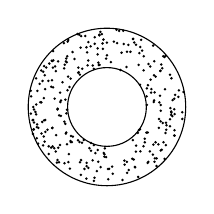
\begin{tikzpicture}[scale=0.5]
				% circles and line
				\draw (0,0) circle (1);
				\draw (0,0) circle (2);
				%\draw (0,0) -- (2,2);
				%\node[thick] at (0,0) {\pgfuseplotmark{o}};
				%markings fro interval
				%\draw[thick] (0.8,0.8) -- (1.6,1.6);
				%\node[rotate=45, thick] at (0.8,0.8) {\pgfuseplotmark{|}};
				%\node[rotate=45, thick] at (1.6,1.6) {\pgfuseplotmark{|}};
				%\node[thick] at (1.2,1.2) {\pgfuseplotmark{*}};
				% labels
				%\node at (1.0,1.4) {$r_\tau$};
%				\node at (1.3,0) {$r_0$};
%				\node at (2.3,0) {$r_1$};
				% random points
				\foreach \x in {1,...,300}{
					\pgfmathsetmacro{\r}{sqrt(random(100,400)/100)}%
					\pgfmathsetmacro{\a}{random(0,360)}%
					\pgfmathsetmacro{\x}{\r*sin(\a)}
					\pgfmathsetmacro{\y}{\r*cos(\a)}
					\node[fill,circle,inner sep=0pt,minimum size=1pt] at (\x ,\y) {};
				}
			\end{tikzpicture}
		\end{subfigure}
		\begin{subfigure}[t]{0.45\textwidth}
			\centering
			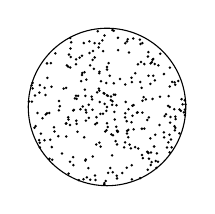
\begin{tikzpicture}[scale=0.5]
				% circles and line
				\draw (0,0) circle (2);
				%\draw (0,0) -- (2,2);
				%\node[thick] at (0,0) {\pgfuseplotmark{o}};
				%markings fro interval
				%\draw[thick] (0.0,0.0) -- (0.8,0.8);
				%\node[rotate=45, thick] at (0.8,0.8) {\pgfuseplotmark{|}};
				%\node[thick] at (0.3,0.3) {\pgfuseplotmark{*}};
				% labels
				%\node at (0.05,0.5) {$r_\tau$};
%				\node at (-0.3,0) {$r_0$};
%				\node at (2.3,0) {$r_1$};
				%\node at (1.0,0.6) {$r_\tau^*$};
				% random points
				\foreach \x in {1,...,300}{
					\pgfmathsetmacro{\r}{sqrt(random(0,400)/100)}%
					\pgfmathsetmacro{\a}{random(0,360)}%
					\pgfmathsetmacro{\x}{\r*sin(\a)}
					\pgfmathsetmacro{\y}{\r*cos(\a)}
					\node[fill,circle,inner sep=0pt,minimum size=1pt] at (\x ,\y) {};
				}
			\end{tikzpicture}
		\end{subfigure}
	\end{figure}
	We call \textbf{Droplet} the support of $\mu_Q$, which in our case is the set of all complex values $z$ such that $r_0 \leq |z| \leq r_1$.
	}
\end{frame}

\begin{frame}
	\only<1-3>{
	Let $\mu \in  \M^1(\C)$ be a measure such that $\dd \mu = \frac{1}{4\pi} (r q'(r))' \delta_{\mathcal{S}} \dd \phi \dd r$.
	\begin{equation*}
		\int_{\C} \dd \mu = 1,
	\end{equation*}
	that is, 
	\begin{equation*}
		r_1 q'(r_1) - r_0 q'(r_0) = 2.
	\end{equation*}
	but $r_0$ is the largest solution of $r q'(r) = 0$ and $r_ 1$ is the smallest solution of $r q'(r) = 2$.\visible<2->{Now, by Euler-Lagrange Theorem, if $\mu$ satisfies that
	\begin{align*}
		2 U^{\mu}(z) & \geq l - Q(z), \quad z \in \C  \\
		2 U^{\mu}(z) & = l - Q(z), \quad z \in \{z \ | \ r_0 \leq |z| \leq r_1\}.
	\end{align*}
	with $I_Q(\mu) < \infty$, then $\mu_Q = \mu$.
	\visible<3>{We must compute
	\begin{equation*}
		U^{\mu}(z) =  \int \ln{|z-t|^{-1}} \dd \mu_Q(t) = \frac{1}{4\pi} \int_{r_0}^{r_1} (r q'(r))'  \int_{-\pi}^{\pi} \ln \frac{1}{|z - r\ee^{\ii \phi}|} \dd \phi \dd r.
	\end{equation*}
	}
	}
	}
	\only<4-7>{
	With the formula
	\begin{equation*}
		\int_{-\pi}^{\pi} \ln \frac{1}{|z - r\ee^{\ii \phi}|} \dd \phi =
		\begin{cases}
			2\pi \ln \frac{1}{r},  \quad |z| \leq r, \\
			2\pi \ln \frac{1}{|z|}, \quad |z| > r.
		\end{cases}
	\end{equation*}
	we can compute $U^\mu(z)$ \visible<5->{for $|z| < r_0$
	\begin{equation*}
		U^{\mu}(z) =  \frac{1}{2} \int_{r_0}^{r_1} (r q'(r))'  \ln \left(\frac{1}{r}\right) \dd r = -\frac{1}{2}(2\ln(r_1) - q(r_1)) - \frac{1}{2}q(r_0),
	\end{equation*} \visible<6->{
	for  $|z| > r_1$
	\begin{equation*}
		U^{\mu}(z) =  \frac{1}{2} \int_{r_0}^{r_1} (r q'(r))'  \ln \left(\frac{1}{z}\right) \dd r = \ln \frac{1}{|z|},
	\end{equation*} \visible<7->{
	 for $r_0 \leq |z| \leq r_1$ 
	\begin{align*}
		U^{\mu}(z) & =  \frac{1}{2} \int_{r_0}^{|z|} (r q'(r))'  \ln \left(\frac{1}{r}\right) \dd r + \frac{1}{2} \int_{|z|}^{r_1} (r q'(r))'  \ln \left(\frac{1}{z}\right) \dd r, \\
		& = -\frac{1}{2}(2 \ln(r_1) - q(r_1)) - \frac{1}{2} q(|z|).
	\end{align*}
	}}}}
	\only<8->{
	Define $l = - (2 \ln(r_1) - q(r_1))$, then
	\begin{equation*}
		2 U^{\mu}(z) =
		\begin{cases}
			l - q(r_0),  \quad |z| < r_0, \\
			2 \ln \frac{1}{|z|}, \quad |z| > r_1, \\
			l - q(|z|), \quad r_0 \leq |z| \leq r_1.
		\end{cases}
	\end{equation*}
	We need to prove that for $z \in \C$, we have $2 U^{\mu}(z) \geq l - q(|z|)$ while on $r_0 \leq |z| \leq r_1$ we have $2 U^{\mu}(z) = l - q(|z|)$.
	\visible<9->{
		\begin{columns}
			\begin{column}{0.5\textwidth}
					\begin{center}
					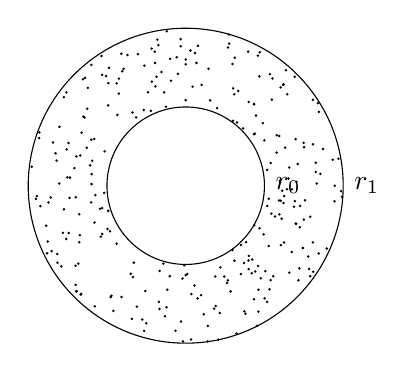
\begin{tikzpicture}[scale=1]
						% circles and line
						\draw (0,0) circle (1);
						\draw (0,0) circle (2);
						%\draw (0,0) -- (2,2);
						%\node[thick] at (0,0) {\pgfuseplotmark{o}};
						%markings fro interval
						%\draw[thick] (0.8,0.8) -- (1.6,1.6);
						%\node[rotate=45, thick] at (0.8,0.8) {\pgfuseplotmark{|}};
						%\node[rotate=45, thick] at (1.6,1.6) {\pgfuseplotmark{|}};
						%\node[thick] at (1.2,1.2) {\pgfuseplotmark{*}};
						% labels
						%\node at (1.0,1.4) {$r_\tau$};
						\node at (1.3,0) {$r_0$};
						\node at (2.3,0) {$r_1$};
						% random points
						\foreach \x in {1,...,300}{
							\pgfmathsetmacro{\r}{sqrt(random(100,400)/100)}%
							\pgfmathsetmacro{\a}{random(0,360)}%
							\pgfmathsetmacro{\x}{\r*sin(\a)}
							\pgfmathsetmacro{\y}{\r*cos(\a)}
							\node[fill,circle,inner sep=0pt,minimum size=1pt] at (\x ,\y) {};
						}
					\end{tikzpicture}
				\end{center}
			\end{column}
			\begin{column}{0.5\textwidth}
				$r_0$ is the biggest $r$ s.t. $rq'(r) = 0$. 
				\begin{align*}
					 q(r_0) \leq q(|z|), \quad |z| < r_0.
				\end{align*}
				$r_1$ is the smallest $r$ s.t. $r q'(r) = 2$. Then,  for $|z| > r_1$ 
				\begin{align*}
					& q(|z|) - 2 \log(|z|) \geq q(r_1) - 2 \log(r_1) \\
					& \implies 2 \ln \frac{1}{|z|} \geq l - q(|z|)
				\end{align*}
			\end{column}
		\end{columns}
	}}
%	Firstly, for $0 < |z| < r_0$ we need that $q(r_0) - q(|z|) \geq 0$ such that $2 U^{\mu}(z) = l - q(r_0)$ is less than or equal to $l - q(|z|)$. This is true because of the growing condition on $q$. Moreover, we need for $|z| > r_1$, that $- 2 \ln |z| + q(|z|) \geq - 2 \ln(r_1) + q(r_1)$. The same argument on the growing of $q$ and $\ln$ holds to state that this is also true. Therefore, $\mu_Q = \mu$ and we have found our equilibrium measure.
\end{frame}

%---------------------------------------------------------